
\documentclass[11pt]{report}

\usepackage{graphicx}
%\graphicspath{ {images/} }

\marginparwidth 0.5in 
\oddsidemargin 0.25in 
\evensidemargin 0.25in 
\marginparsep 0.25in
\topmargin 0.0in 
\textwidth 6in \textheight 8.5in

\title{sQuire: A Web Based Collaborative Editor}
\author{Kevin Benzing, Ben Bolton, Robert Carlson, Feng Guan, Brandon Jank, Wyatt Knickerbocker, Kevin Morales, Brandon Ratcliff}
\author{benz5834, bolt1003, carl7595, guan2264, jank6275, knic1468, mora5651, ratc8795}

\begin{document}

\maketitle

\tableofcontents

\chapter{Application Domain Specification}

\section{Program Premise}
\begin{figure}[h!]
\caption{Squire will be a web-based collaborative text editor that compiles java code in throwaway "rooms". Multiple users can edit and communicate in real time.}
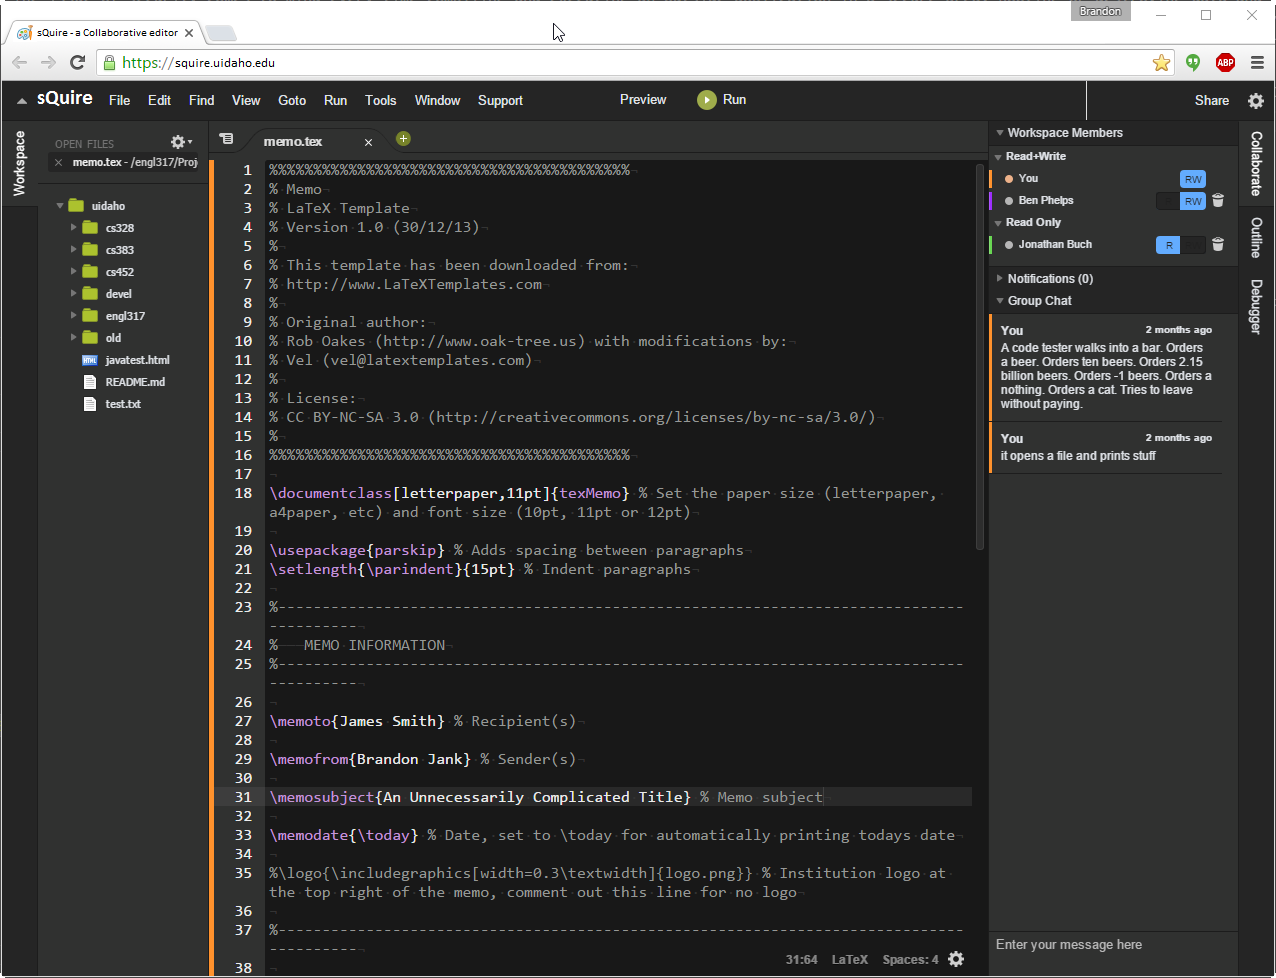
\includegraphics[width=0.7\textwidth]{squire}
\end{figure}

\subsection{Core Features (carl7595)}
\begin{itemize}
  \item Web based
  \item Some Common IDE features
  \item Collaborative tools
  \item Encapsulated Workspaces
  \item Compile and Download
  \item Self Destructing Rooms
\end{itemize}
The central idea behind sQuire is a somewhat akin to a code hostel. A collaborative editor which provides private, but shareable on demand spaces, with a low overhead for creation and ease of use. These spaces are meant for short term use, over an indeterminate period. Once the collaboration is done, the space is cleared and made available for others to use.

With this vision in mind, sQuire best accomodates its users by being a browser based application. There should be no need for a user to download a client program, which would require periodic updates and ultimately require deletion on the users' end. By doing all of the collaboration and storage on a central server, accessed by the browser, we can make it more accessible to a wider audience. It may also encourage the development of collaborative "toy" projects by making it easier to start project spaces and find assistance when a project stalls.

sQuire will be focused on coding in the Java language, though there are many worthwhile languages to choose from. Focusing on a single language will allow us to add more IDE-like features to assist in collaboration and make the language more accessible to those learning it.
IDE-like Features:
\begin{itemize}
  \item Key word color coding
  \item Parenthesis mismatch detection
  \item Missing end of line detection/prompting
\end{itemize}

sQuire is a collaborative tool, rather than a fully featured IDE with step through run-time debugging. Its features should be geared towards making it easier to debug code collaboratively, in the browser, without over-reliance on other tools. At a minimum, it needs:
\begin{itemize}
  \item Native chat functionality
  \item Author attribution for code (colored underlining, footnote, etc.)
  \item Ability to "jump to" another user's cursor
  \item Ability to import/export code as plain text
  \item Account based access to projects
\end{itemize}

Collaborative features that would be "nice":
\begin{itemize}
  \item Ability to save/restore to "snapshots" of the project
  \item Achievement and statistic tracking
\end{itemize}

User workspaces will be encapsulated, for both security and privacy. This could be accomplished using a container solution such as Docker or lmctfy (a free Google version). Containers have a lower performance hit to the host server than virtual machines, which are also a commonly implemented solution.  

While security is a concern, we hope to address this using user space encapsulation, and by not running user code on the server. When users compile code, the compiled jar is downloaded and run locally from their own machines. While this means users are responsible for vetting the function of the code before running it on their machines, it means that our server resources are not being used as part of a bot net or similar exploit.

Finally rooms must be self-destructing. For the convenience of the user, deletion of the space should be automatic after an appropriate period of inactivity. While a notification email should be sent to the space owner prior to deletion, again no user intervention should be required.

\subsection{Storage and Organization (benz5834)}
The squire program will have a top down directory structure.
Under the top domain, each individual registered user will have the ability to create projects (rooms) where they can build their program. 
Inside the room the user will be able to create any number of files or pages to keep track of their project. 
They will also have the ability to import and export files to and from their own machine and the project. 
After creation the user will be able to switch between projects and create and delete pages from within the project itself.  
They will have the ability to share their projects and invite other users to read or edit their work. 
All of the user data, as well as each user’s relevant project and page information, as well as who has access to each project will be stored and maintained by a MySQL database.

\subsection{Security Nightmare (jank6275)}
The issue of security comes to mind every time compiling and executing an outside application in a secure area. Rooting or destroying data and infrastructure is trivial when you are freely allowed to execute arbitrary Java. In order to allow for this functionality we must implement some type of security strategy. We could limit or block functionality in Java which is a cat and mouse game that breaks usability. We could compile and execute code on the client side. This would require a compiler written in JavaScript and cause compatibility issues on certain clients with reduced permissions or an exotic build environment. Or we could just Docker.


Docker allows us to create containers that contain not only the user's build environment, but the server infrastructure to host their project. Containers include the application and all of its dependencies, but share the kernel with other containers. Simply put, users can destroy their own containers but nobody else’s. Obviously we will want to harden against known and obvious vectors, but at least any damage a user can do is limited to their own project. Containerization also allows us to take snapshots so that even if something goes wrong, we can always revert back to a working state.

\subsection{Execution (guan2264)}
The Squire program will have a browser based client. Squire users can use this client to login their account, manipulate their project, and logout. The Squire editor will run clientside through Ace. Ace is an embeddable code editor written in JavaScript. It can be easily embedded in any web page, JavaScript application, and browser based client. On the other hand, the user data, user project, and edit information will saved in a MySQL database on the owner's hard drive.  

\subsection{Collaboration (ratc8795)}
The code editor will be a collaborative editor. Multiple users can edit the same file at the same time. This means that any changes one user makes need to be synced to the server, and then to the editors of any other users editing the same file. Some research shows that all popular collaborate editors (Google Docs, Cloud 9, etc) use an algorithm called Operational Transformation. On a basic level, this algorithm works by treating every change to a file as either an insert command, or a delete command. These commands are synced across clients to keep the file state the same. Squire will need something similar. It looks like there are several open source implementations of this algorithm, notably OT.js. These may or may not be adequate for use in Squire.
 
\subsection{Achievement System (ratc8795)}
In order to make Squire interesting, but still retain its usability, Squire will contain an achievement system. Achievements will be publicly visible to all users in the user's profile. When a user gains an achievement, it will be announced in the project chat. Achievements should be fun, and should be obtainable just by writing code (i.e, users shouldn’t have to actively try to get achievements). Some possible achievements: Lucky Break (a file compiles successfully on the first try), Social Butterfly (a user joins a project that has 10+ users), Job Security (Write a 1000+ line file without any comments).

\subsection{Permissions System (bolt1003)}
Squire will have a permissions system that encompasses files, folders, users and rooms. The administrator will have the ability to delegate permission to other users.  The administrator will have the ability to set global permissions to users to control read, write, execute, room creation and sharing.  Each room with have its own set of permissions. These permissions are controlled by the moderator that is assigned to that room and the administrator. By default the creator of the room is the moderator of the room but this duty can be delegated to another if desired. The system has three default user groups, Administrator, Moderators and Users. Users have the ability to read, write and execute code by default. Moderators have the ability to manage rooms by adding or removing users to their rooms, creating sub-rooms and managing moderators for those rooms. Administrators have all encompassing power over all permissions in the system.

\subsection{Interface Structure (mora5651)}
Since sQuire is an online collaborative editor, and interface structure plays a key roll in organizing all the features to fit properly. We decided in using Cloud9's interface as a base for sQuire's interface layout/structure. Cloud9 incorporates many of the same features as sQuire including file management, editor, and chat options. Other collaborative IDEs to consider Floobits, Kobra, and Codebox. 

\subsection{Chat System (knic1468)}
We will most likely use a websocket-based chat system for sQuire, as it allows the easiest modification; Users and their coded colors will be listed, and their names next to their chat lines. The goal is to make a simple and lightweight, secure chat that allows users to collaborate with each other in an area outside the workspace.




\section{Application Domain Study}
\subsection{codepad.org (jank6275)}
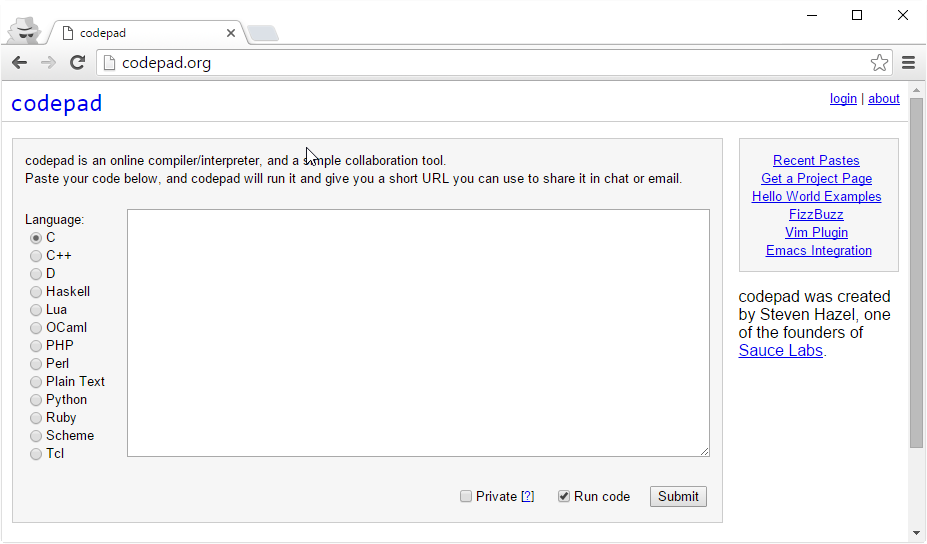
\includegraphics[width=\textwidth]{codepad}
Codepad is an online compiler and simple collaboration tool that compiles interactive code from the web. Safely compiling and executing arbitrary code from the web will always be a security problem. Steven Hazel, the creator of codepad.org, used Docker to containerize each development environment and then execute the user’s code. This limits the damage an unwitting or malicious user can do to just their container. We should utilize this technology with sQuire. The webserver, database, front-end, and user application can be copied from a template and a virtual machine spun up just for that user’s project.


Even though codepad.org uses cool technology for solving the security issue, it is not without its flaws. There is no live chat functionality and communication is critical for online collaboration. You cannot edit code with someone at the same time, you can only save-and-share. This slows down the development process and can cause code "collisions". These areas are a niche for sQuire to shine in among a large swath of online collaborative IDEs.

\subsection{Cloud9 IDE - c9.io (guan2264)}
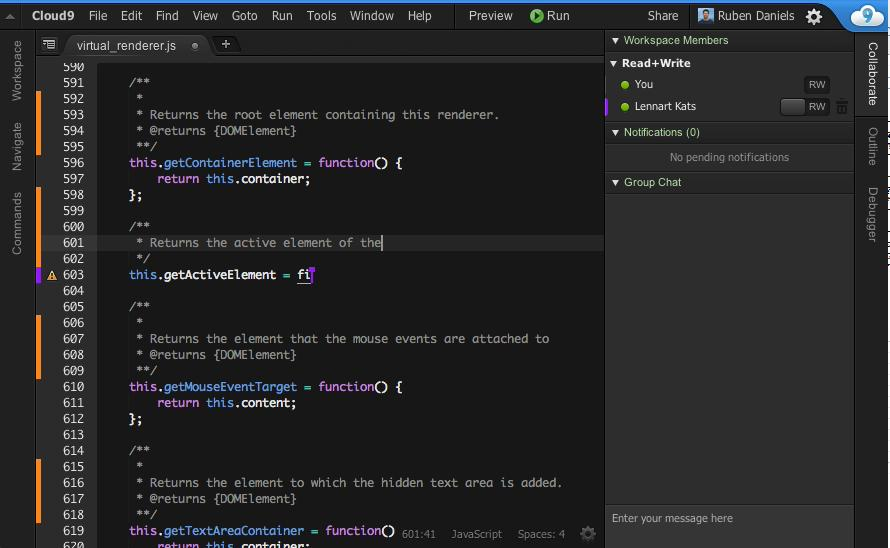
\includegraphics[width=\textwidth]{cloud9}
Cloud9 IDE is a freeware online integrated development environment. It supports hundreds of programming languages, including PHP, Ruby, Perl, Python, and JavaScript. It enables users to get started with coding immediately with pre-setup work spaces, collaborate with their peers with collaborative coding features, and web development features like live preview and browser compatibility testing. It is written almost entirely in JavaScript, and uses Node.js on the back-end. The editor component uses Ace. 

\subsection{IDEone (ratc8795)}
Ideone (ideone.com) is a online compiling and debugging system. It allows online compiling and debugging of over 60 languages. It is implemented using Sphere-engine's api. Sphere-engine provides a system to allow execution of untrusted code. This is reflected in Ideone. For example, when you try and run a program that does the equivalent of "sleep 60", "ping google.com", or "rm -rf /", an error is thrown and the code is not run. Ideone is extremely simple. It provides a basic code editor, an option to select the language, a box to type in any standard input, and an output box showing any errors or output. It also provides functionality to save and share scripts with other people. Notable limitations are that there is only one file, and no collaborative editing. As far as a simple way to execute code from many different languages, Ideone does a very good job.

\subsection{Codenvy (bolt1003)}
Codenvy is an online IDE that supports a variety of languages. This includes C, C++, Go, Python, Java, JavaScript, PHP and Ruby. Codenvy has a dedicated virtual machine per project (implemented using docker) to compile and execute code within. Codenvy allows for multiuser editing of code in real-time. Codenvy allows a user to create a temporary clone of a project to modify and execute in its own dedicated VM. Codenvy integrates with popular subversion control systems and hosting such as GitHub. SSH is provided so that users can login to the VM directly to make modification and execute code.


Codenvy provides basic features free of charge, most of which would be fine for moderate use by a single user or small group.  Their business model is targeted at larger business so premium features come at a premium. The integrated interpreter is difficult to setup initially and often provides cryptic error messages. Logging in via ssh and executing code is more consistent experience. Codenvy lacks an integrated chat client so a third party client is needed.

\subsection{Floobits (mora5651)}
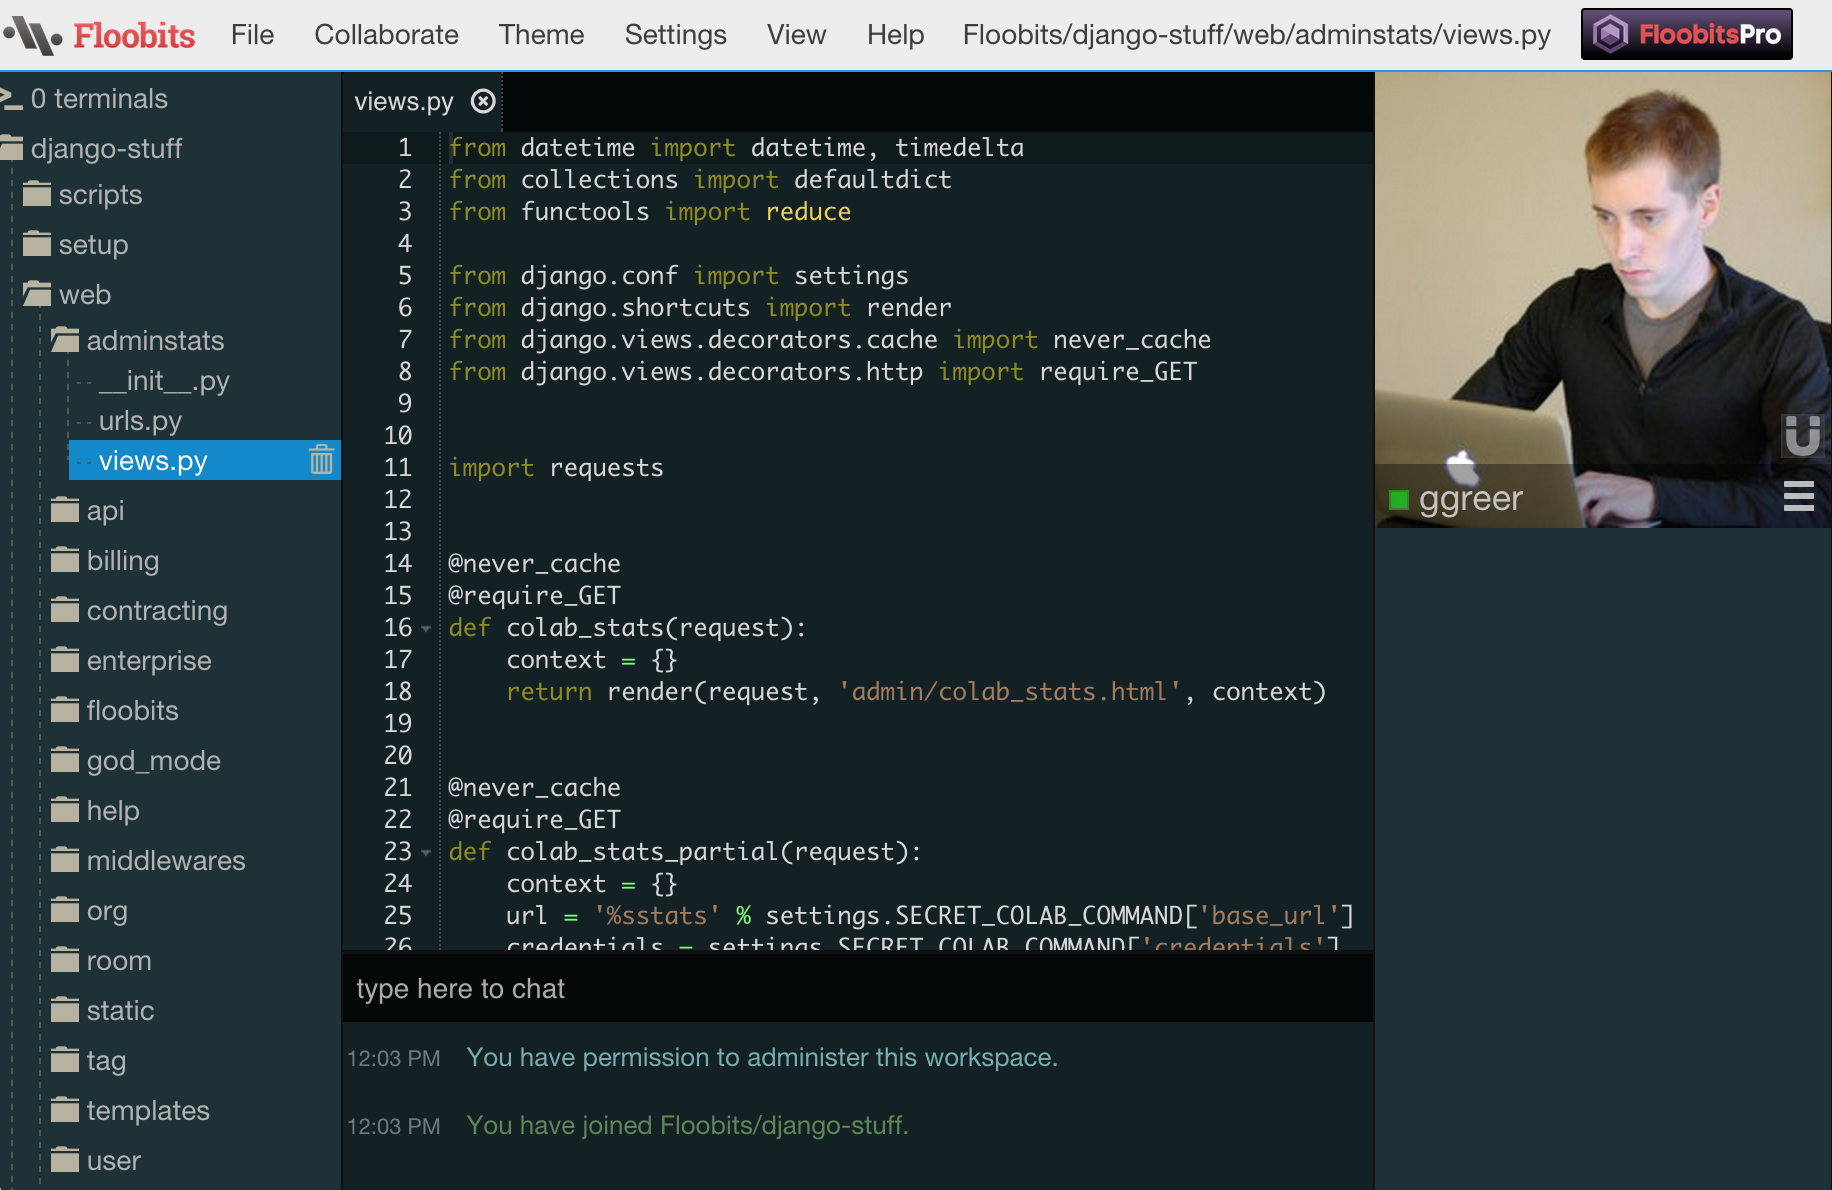
\includegraphics[width=\textwidth]{Floobits}
Floobits is a web based application that allows users to collaborate on the same code while using there favorite editor. Examples of editors that are supported in Floobits include Emacs, Sublime, Atom, and more. Although Floobits focuses towards "paired programming" it also supports multi user groups integrating voice chat, as well as a video chat options using Google Hangouts. Floobits is fairly simple to customize giving the users options to install different plugins for different functionality Floobits has to offer. However, to access some of these features you will need an upgraded paided account. Floobits also suffers from security issues.

\subsection{Google Docs (benz5834)}
Google Docs is a collaborative document editor built around the Google ecosystem. Anyone with an account can create documents, spreadsheets, slideshows, and forms. Within each one of these documents there is a menu to share your document and even give editing privileges. In this sense it is very similar to what we want to accomplish with Squire. Account based document creation with the ability to collaborate and work together on the same document at the same time. There are even a few features that google docs has that our squire program could benefit from. A running comment thread within each document allows for editors and viewers to be able to leave notes and comments about what they have done outside of the document itself. There are a large number of document templates included within each document type as well. The project management page is also very clean and easy to organize with both a list and grid view of saved documents. And because accounts are tied in with email addresses, it is very easy to send messages to collaborators about your documents. Google Docs is well used for every type of user so I think it is a very important tool to study while creating Squire.

\subsection{Sharelatex (carl7595)}
Sharelatex is a collaborative text editor targeted towards the Latex language. Sharelatex.com uses a similar email based registration scheme, and does allow for compiling in the browser. It also includes a history feature of changes made to the document, which is one way that snapshots could be added at working compile. I particularly like that in the interface there is a share button that immediately prompted for the email address of the person you want to share with. The chat window is a pane that opens on the right side, squeezing the rest of the windows to accomodate this. This is not a problem in full screen mode, but I think I would prefer the chat to be always open and near the bottom of the screen. It has an option for creating a sample project, which would be a great feature for giving someone a template container to work with to make things more accessible to new coders. 

\subsection{Mibbit and Ratchet (knic1468)}
Because sQuire will require a chat function to truly be a collaborative IDE, I took a look at two lightweight chat clients, mibbit and the demo on Ratchet. Both were lightweight, but one used irc protocols and connected to servers, while Ratchet is websocket based, and the chat rooms can be more custom and hosted on the local server. Since the Ratchet demo is a simple example of the Ratchet API, it allows one to really see what it can let you do. As a PHP-based API, it is developed for being browser-based as well. While not as lightweight as a built-in irc client, the websocket-based client would be more secure and modifiable.



\section{Use Case Descriptions}
\subsection{Open project chat (jank6275)}
\begin{tabular}{ p{2cm} p{12cm} }
 \hline
 \\
 \textit{Actors:} & User \\ 
 \\
 \textit{Goals:} & To open the project chat window. \\
 \\
 \textit{Pre-conditions:} & User must be registered, signed in, and in editor Mode.  \\
 \\
 \textit{Summary:} & User clicks on open project chat and the chat opens, displaying chat history and updating when needed. \\ 
 \\
 \textit{Related use cases:} & Join global chat. \\ 
 \\
 \textit{Steps:} & \begin{enumerate}
  \item User clicks open project chat.
  \item Chat is notified that user has joined.
  \item System displays project chat window.
 \end{enumerate} \\
 \\
 \textit{Alternatives:} & None. \\
 \\
 \textit{Post-conditions:} & None. \\
 \\
\hline
\end{tabular}

\subsection{Open global chat (jank6275)}
\begin{tabular}{ p{2cm} p{12cm} }
 \hline
 \\
 \textit{Actors:} & User \\ 
 \\
 \textit{Goals:} & To open the global chat window. \\
 \\
 \textit{Pre-conditions:} & User must be registered, signed in, and anywhere on website.  \\
 \\
 \textit{Summary:} & User clicks on open global chat and the chat opens, displaying chat history and updating when needed. \\ 
 \\
 \textit{Related use cases:} & Join project chat. \\ 
 \\
 \textit{Steps:} & \begin{enumerate}
  \item User clicks open global chat.
  \item Chat is notified that user has joined.
  \item System displays global chat window.
 \end{enumerate} \\
 \\
 \textit{Alternatives:} & None. \\
 \\
 \textit{Post-conditions:} & None. \\
 \\
\hline
\end{tabular}

\subsection{Close project chat (jank6275)}
\begin{tabular}{ p{2cm} p{12cm} }
 \hline
 \\
 \textit{Actors:} & User \\ 
 \\
 \textit{Goals:} & To close the project chat window. \\
 \\
 \textit{Pre-conditions:} & User must be registered, signed in, and in editor Mode.  \\
 \\
 \textit{Summary:} & User clicks on close project chat and the chat window closes. \\ 
 \\
 \textit{Related use cases:} & Close global chat. \\ 
 \\
 \textit{Steps:} & \begin{enumerate}
  \item User clicks close project chat.
  \item Chat is notified that user has left.
  \item Client closes project chat window.
 \end{enumerate} \\
 \\
 \textit{Alternatives:} & None. \\
 \\
 \textit{Post-conditions:} & None. \\
 \\
\hline
\end{tabular}

\subsection{Close global chat (jank6275)}
\begin{tabular}{ p{2cm} p{12cm} }
 \hline
 \\
 \textit{Actors:} & User \\ 
 \\
 \textit{Goals:} & To close the global chat window. \\
 \\
 \textit{Pre-conditions:} & User must be registered, signed in, and anywhere on website.  \\
 \\
 \textit{Summary:} & User clicks on open global chat and the chat opens, displaying chat history and updating when needed. \\ 
 \\
 \textit{Related use cases:} & Close project chat. \\ 
 \\
 \textit{Steps:} & \begin{enumerate}
  \item User clicks close global chat.
  \item Chat is notified that user has left.
  \item Client closes global chat window.
 \end{enumerate} \\
 \\
 \textit{Alternatives:} & None. \\
 \\
 \textit{Post-conditions:} & None. \\
 \\
\hline
\end{tabular}

\subsection{Write to project chat (jank6275)}
\begin{tabular}{ p{2cm} p{12cm} }
 \hline
 \\
 \textit{Actors:} & User \\ 
 \\
 \textit{Goals:} & To send text to project chat. \\
 \\
 \textit{Pre-conditions:} & User must be registered, signed in, a project opened, with the project chat window open, and the text box selected.  \\
 \\
 \textit{Summary:} & User clicks in the project chat text box and then types a message then either presses enter or clicks the submit button. The text is displayed to all users in the chat, including the user. \\ 
 \\
 \textit{Related use cases:} & Write to global chat. \\ 
 \\
 \textit{Steps:} & \begin{enumerate}
  \item User clicks in the project chat box.
  \item User types a message and then presses enter or clicks submit button.
  \item Message is relayed to all clients with project chat open.
  \item Message is displayed.
 \end{enumerate} \\
 \\
 \textit{Alternatives:} & None. \\
 \\
 \textit{Post-conditions:} & None. \\
 \\
\hline
\end{tabular}

\subsection{Write to global chat (jank6275)}
\begin{tabular}{ p{2cm} p{12cm} }
 \hline
 \\
 \textit{Actors:} & User \\ 
 \\
 \textit{Goals:} & To send text to global chat. \\
 \\
 \textit{Pre-conditions:} & User must be registered, signed in, anywhere on website, with the global chat window open, and the text box selected.  \\
 \\
 \textit{Summary:} & User clicks in the global chat text box and then types a message then either presses enter or clicks the submit button. The text is displayed to all users in the chat, including the user. \\ 
 \\
 \textit{Related use cases:} & Write to project chat. \\ 
 \\
 \textit{Steps:} & \begin{enumerate}
  \item User clicks in the global chat box.
  \item User types a message and then presses enter or clicks submit button.
  \item Message is relayed to all clients with global chat open.
  \item Message is displayed.
 \end{enumerate} \\
 \\
 \textit{Alternatives:} & None. \\
 \\
 \textit{Post-conditions:} & None. \\
 \\
\hline
\end{tabular}

\subsection{Modify chat font (jank6275)}
\begin{tabular}{ p{2cm} p{12cm} }
 \hline
 \\
 \textit{Actors:} & User \\ 
 \\
 \textit{Goals:} & To change a users font style inside the global and project chat. \\
 \\
 \textit{Pre-conditions:} & User must be registered, signed in, the user settings window opened, and the chat settings tab open.  \\
 \\
 \textit{Summary:} & The user clicks the settings menu and changes their font style for both the project and global chat through a drop down box of available fonts. \\ 
 \\
 \textit{Related use cases:} & Modify chat color. \\ 
 \\
 \textit{Steps:} & \begin{enumerate}
  \item User clicks the settings menu.
  \item User clicks chat settings tab.
  \item User clicks chat font drop down box.
  \item User clicks desired font.
  \item User clicks save.
  \item The user's selection is saved in the database.
  \item All further chat messages will use the selected font.
 \end{enumerate} \\
 \\
 \textit{Alternatives:} & None. \\
 \\
 \textit{Post-conditions:} & None. \\
 \\
\hline
\end{tabular}

\subsection{Modify chat color (jank6275)}
\begin{tabular}{ p{2cm} p{12cm} }
 \hline
 \\
 \textit{Actors:} & User \\ 
 \\
 \textit{Goals:} & To change a users font color inside the global and project chat. \\
 \\
 \textit{Pre-conditions:} & User must be registered, signed in, the user settings window opened, and the chat settings tab open.  \\
 \\
 \textit{Summary:} & The user clicks the settings menu and changes their font color for both the project and global chat through a drop down box of available colors. \\ 
 \\
 \textit{Related use cases:} & Modify chat font. \\ 
 \\
 \textit{Steps:} & \begin{enumerate}
  \item User clicks the settings menu.
  \item User clicks chat settings tab.
  \item User clicks chat color drop down box.
  \item User clicks desired color.
  \item User clicks save.
  \item The user's selection is saved in the database.
  \item All further chat messages from the user will use the selected color.
 \end{enumerate} \\
 \\
 \textit{Alternatives:} & None. \\
 \\
 \textit{Post-conditions:} & None. \\
 \\
\hline
\end{tabular}

\subsection{Create Project (bolt1003)}
\begin{tabular}{ p{2cm} p{12cm} }
 \hline
 \\
 \textit{Actors:} & Users of sQuire. \\ 
 \\
 \textit{Goals:} & Create a Project. \\
 \\
 \textit{Pre-conditions:} & The user is logged in. \\
 \\
 \textit{Summary:} & User opens the project manager and creates a project. \\ 
 \\
 \textit{Related use cases:} & None. \\ 
 \\
 \textit{Steps:} & \begin{enumerate}
  \item User selects the project manager from the main menu.
  \item User selects open.
  \item Create new project is selected from the task bar.
  \item A name is choosen for the project.
  \item A location is selected for the project.
  \item Language is selected from a drop down menu.
  \item User clicks finish.
 \end{enumerate} \\
 \\
 \textit{Alternatives:} & None. \\
 \\
 \textit{Post-conditions:} & None. \\
 \\
\hline
\end{tabular}

\subsection{Choose Project (bolt1003)}
\begin{tabular}{ p{2cm} p{12cm} }
 \hline
 \\
 \textit{Actors:} & Users of sQuire. \\ 
 \\
 \textit{Goals:} & Open a Project. \\
 \\
 \textit{Pre-conditions:} & A project has been created and the user is logged in. \\
 \\
 \textit{Summary:} & User looks through the list of project and selects the desired project. \\ 
 \\
 \textit{Related use cases:} & None. \\ 
 \\
 \textit{Steps:} & \begin{enumerate}
  \item User selects the project manager from the main menu.
  \item User selects open.
  \item User selects the desired project.
  \item User clicks open in the list of options.
 \end{enumerate} \\
 \\
 \textit{Alternatives:} & None. \\
 \\
 \textit{Post-conditions:} & None. \\
 \\
\hline
\end{tabular}

\subsection{View User Profile(bolt1003)}
\begin{tabular}{ p{2cm} p{12cm} }
 \hline
 \\
 \textit{Actors:} & Users of sQuire. \\ 
 \\
 \textit{Goals:} & Users looks at their profile page. \\
 \\
 \textit{Pre-conditions:} & The user has an account and is logged in. \\
 \\
 \textit{Summary:} & User opens their profile from the main menu to view.\\ 
 \\
 \textit{Related use cases:} & User modifies their profile. \\ 
 \\
 \textit{Steps:} & \begin{enumerate}
  \item The user selects their profile picture from the main menu.
  \item The user selects view Profile from the drop down menu.
 \end{enumerate} \\
 \\
 \textit{Alternatives:} & None. \\
 \\
 \textit{Post-conditions:} & None. \\
 \\
\hline
\end{tabular}

\subsection{Modify User Profile(bolt1003)}
\begin{tabular}{ p{2cm} p{12cm} }
 \hline
 \\
 \textit{Actors:} & Users of sQuire. \\ 
 \\
 \textit{Goals:} & Users updates their profile. \\
 \\
 \textit{Pre-conditions:} & The user is on the view profile page. \\
 \\
 \textit{Summary:} & User modifies their profile information.\\ 
 \\
 \textit{Related use cases:} & None. \\ 
 \\
 \textit{Steps:} & \begin{enumerate}
  \item The user selects modify. 
  \item The user changes their username.
  \item The user clicks update.
  \item The user updates their contact email.
  \item The user clicks update.
  \item The user changes their "About me" information
  \item The user clicks update.
  \item The user clicks finish to disable modify.
 \end{enumerate} \\
 \\
 \textit{Alternatives:} & None. \\
 \\
 \textit{Post-conditions:} & None. \\
 \\
\hline
\end{tabular}

\subsection{Login (guan2264)}
\begin{tabular}{ p{2cm} p{12cm} }
 \hline
 \\
 \textit{Actors:} & Squire User \\ 
 \\
 \textit{Goals:} & Allows user to login to the system and use functions of the system. \\
 \\
 \textit{Pre-conditions:} & The user must have user account. \\
 \\
 \textit{Summary:} & User types in the correct user name and password, click the login button, and login to the system. When login successfully, the system will display the access page for user. \\ 
 \\
 \textit{Related use cases:} & Choose project, create project, join project, delete project, edit project, invite user to project, accept invite to project, remove user from project, project chat, global chat, roject permissions, user preferences, import file, export file, gain achivement, view user profile, and logout. \\ 
 \\
 \textit{Steps:} & \begin{enumerate}
  \item The system displays the Login page that asks the user to enter username and password.
  \item The user types in their username and password.
  \item The user click the login button.
  \item The system checks the username and password from the data base.
  \item The system verifies username and password.
  \item	The system displays the access page for the user.
 \end{enumerate} \\
 \\
 \textit{Alternatives:} & If the user do not enter the correct username and password, the system will ask the user to enter the correct username and password \\
 \\
 \textit{Post-conditions:} & User logs in and use functions of the system. \\
 \\
\hline
\end{tabular}

\subsection{Logout (guan2264)}
\begin{tabular}{ p{2cm} p{12cm} }
 \hline
 \\
 \textit{Actors:} & Squire User \\ 
 \\
 \textit{Goals:} & Allows user to logout to the system. \\
 \\
 \textit{Pre-conditions:} & The user must have user account and already login to the system. \\
 \\
 \textit{Summary:} & User click the logout button and their session is terminated. \\ 
 \\
 \textit{Related use cases:} & Close project chat, close global chat, close project file, and login. \\ 
 \\
 \textit{Steps:} & \begin{enumerate}
  \item The user click the logout button.
  \item The system invalidates the session.
  \item The system logs the user out.
  \item The system redirects to the default login page.
 \end{enumerate} \\
 \\
 \textit{Alternatives:} & None\\
 \\
 \textit{Post-conditions:} & User's previous session is terminated and the system displays the login page. \\
 \\
\hline
\end{tabular}

\subsection{Invite user to project (ratc8795)}
\begin{tabular}{ p{2cm} p{12cm} }
 \hline
 \\
 \textit{Actors:} & User sending invites, user receiving invites \\ 
 \\
 \textit{Goals:} & Give another user access to a project. \\
 \\
 \textit{Pre-conditions:} & User has the permissions necessary to invite a user to a project. \\
 \\
 \textit{Summary:} & User opens a dialog to invite users, inputs one or more users, and the level of access to the project that they should be given. \\ 
 \\
 \textit{Related use cases:} & Accept invite to project,  project permissions \\ 
 \\
 \textit{Steps:} & \begin{enumerate}
  \item User clicks on a button to invite users.
  \item A dialog is displayed to the user.
  \item User types in one or more emails.
  \item User specifies the level of access for each user.
  \item User clicks submit.
  \item The dialog disappears.
  \item Emails are sent to the email addresses specified containing invites.
 \end{enumerate} \\
 \\
 \textit{Alternatives:} & User does not have permission to invite others to the project, so the button to invite users is not displayed. \\
 \\
 \textit{Post-conditions:} & None. \\
 \\
\hline
\end{tabular}

\subsection{Edit project file (ratc8795)}
\begin{tabular}{ p{2cm} p{12cm} }
 \hline
 \\
 \textit{Actors:} & One or more users editing a file \\ 
 \\
 \textit{Goals:} & Make changes to a file and sync those changes with other users editing the same file. \\
 \\
 \textit{Pre-conditions:} & User has the permissions necessary to edit the project, and the file is open.\\
 \\
 \textit{Summary:} & A user makes a change to a file in a text editor, and those changes are reflected to other users editing the same file. \\ 
 \\
 \textit{Related use cases:} & None. \\ 
 \\
 \textit{Steps:} & \begin{enumerate}
  \item User makes a change in the editor.
  \item The editor of other users editing the same file reflects the change
  \item The editor updates any syntax highlighting and formatting
  \item A note in the margin updates to show the user was the last one to edit that line
  \item The editor of other users editing the same file shows the same note in the margin
 \end{enumerate} \\
 \\
 \textit{Alternatives:} & User does not have permission to edit the file, so the editor ignores any input from that user. \\
 \\
 \textit{Post-conditions:} & None. \\
 \\
\hline
\end{tabular}

\subsection{Open project file (ratc8795)}
\begin{tabular}{ p{2cm} p{12cm} }
 \hline
 \\
 \textit{actors:} & User \\ 
 \\
 \textit{goals:} & A user selects a file from the project for editing or viewing. \\
 \\
 \textit{pre-conditions:} & The file already exists \\
 \\
 \textit{summary:} & A user selects a file from the project which opens, replacing any file that is already open. \\ 
 \\
 \textit{related use cases:} & Close a project file \\ 
 \\
 \textit{steps:} & \begin{enumerate}
  \item A user selects a file from the list of files in the project.
  \item If a file is currently open, that file is closed.
  \item The file is opened in the editor.
  \item The editor shows the user as being active in the file.
 \end{enumerate} \\
 \\
 \textit{alternatives:} & None. \\
 \\
 \textit{post-conditions:} & None. \\
 \\
\hline
\end{tabular}

\subsection{Close a project file (ratc8795)}
\begin{tabular}{ p{2cm} p{12cm} }
 \hline
 \\
 \textit{actors:} & User \\ 
 \\
 \textit{goals:} & Closing a file. \\
 \\
 \textit{pre-conditions:} & A user clicks a button to close an open file and the editor is closed. \\
 \\
 \textit{summary:} & The file is closed. \\ 
 \\
 \textit{related use cases:} & Open a file. \\ 
 \\
 \textit{steps:} & \begin{enumerate}
  \item A user clicks on a button to close the file, or has selected another file to open.
  \item The file is closed, and removed from the editor.
  \item The editor now longer shows the user as being active in the file.
 \end{enumerate} \\
 \\
 \textit{alternatives:} & none. \\
 \\
 \textit{post-conditions:} & none. \\
 \\
\hline
\end{tabular}

\subsection{Create a project file (ratc8795)}
\begin{tabular}{ p{2cm} p{12cm} }
 \hline
 \\
 \textit{actors:} & User \\ 
 \\
 \textit{goals:} & Creating a new file. \\
 \\
 \textit{pre-conditions:} & The user has permission to create a new file. \\
 \\
 \textit{summary:} & A user new project file is cr \\ 
 \\
 \textit{related use cases:} & Move a file, Delete a file \\ 
 \\
 \textit{steps:} & \begin{enumerate}
  \item A user clicks on a button to create a file.
  \item A dialog is displayed asking for a file path.
  \item The user types in the file path.
  \item The file is created.
 \end{enumerate} \\
 \\
 \textit{alternatives:} & The specified file name contains invalid characters, so an error is displayed. \\
 \\
 \textit{post-conditions:} & None. \\
 \\
\hline
\end{tabular}

\subsection{Move a file (ratc8795)}
\begin{tabular}{ p{2cm} p{12cm} }
 \hline
 \\
 \textit{actors:} & User \\ 
 \\
 \textit{goals:} & A user moved from one location to another\\
 \\
 \textit{pre-conditions:} & The user has permission to move a file. \\
 \\
 \textit{summary:} & A file is moved from it's location to a new location specified by the user \\ 
 \\
 \textit{related use cases:} & Create a file, Delete a file \\ 
 \\
 \textit{steps:} & \begin{enumerate}
  \item A user clicks on a button next to a file to rename it
  \item A dialog is displayed asking for a file name.
  \item The user types in the file name.
  \item The file is moved to the new location
 \end{enumerate} \\
 \\
 \textit{alternatives:} & The user types in a location that is invalid; an error is displayed. \\
 \\
 \textit{post-conditions:} & None. \\
 \\
\hline
\end{tabular}

\subsection{Delete a file (ratc8795)}
\begin{tabular}{ p{2cm} p{12cm} }
 \hline
 \\
 \textit{actors:} & User \\ 
 \\
 \textit{goals:} & A file is deleted \\
 \\
 \textit{pre-conditions:} & The user has permission to delete a file. \\
 \\
 \textit{summary:} & A user clicks a button to delete a file, and it is removed from the project \\ 
 \\
 \textit{related use cases:} & Create a file, Delete a file \\ 
 \\
 \textit{steps:} & \begin{enumerate}
  \item A user clicks on a button next to a file to delete it
  \item A dialog is displayed asking for confirmation.
  \item The user clicks yes.
  \item The file is deleted.
 \end{enumerate} \\
 \\
 \textit{alternatives:} & The user clicks no in the confirmation so the file is not deleted. \\
 \\
 \textit{post-conditions:} & None. \\
 \\
\hline
\end{tabular}

\subsection{Gain an achievement (ratc8795)}
\begin{tabular}{ p{2cm} p{12cm} }
 \hline
 \\
 \textit{actors:} & User \\ 
 \\
 \textit{goals:} & Notify the user that they gained an achievement \\
 \\
 \textit{pre-conditions:} & The user has met the requirements for the achievement. \\
 \\
 \textit{summary:} & A user is informed that the earned an achievement, and users in the project chat are informed that the user earned an achievement, and the user's profile is updated to include the achievement \\ 
 \\
 \textit{related use cases:} & None. \\ 
 \\
 \textit{steps:} & \begin{enumerate}
  \item A user earns an achievement.
  \item A pop up is displayed to the user informing them of the achievement.
  \item After a couple seconds, the pop up goes away.
  \item A message is sent to the group chat informing other users of the achievement.
 \end{enumerate} \\
 \\
 \textit{alternatives:} & None. \\
 \\
 \textit{post-conditions:} & None. \\
 \\
\hline
\end{tabular}

\subsection{Join Project(mora5651)}
\begin{tabular}{ p{2cm} p{12cm} }
\hline
\\
\textit{Actors:} & User.\\
\\
\textit{Goals:} & To join an existing project.\\
\\
\textit{Pre-conditions:} & Must be registered, logged in, then must choose a project to join.\\
\\
\textit{Summary:} & User has logged in, user then chooses a project to join, if user is allowed then the user joins the project. \\
\\
\textit{Related use cases:} & Invite user to project, Accept user invite. \\
\\
\textit{Steps:} & \begin{enumerate}
 \item The user chooses the "join a project" button. 
 \item If the project is held in a public room then the user joins. 
 \item If the project is held in a private room then the user will need permission. 
 \item If the admin of the project the user wants to join is accepted. Then the user joins the project. 
\end{enumerate}\\
\\
\textit{Alternatives:} & User may decline an inventation to join a project. \\
\\
\textit{Post-conditions:} & You entered a Project. \\
\\
\hline
\end{tabular}

\subsection{Delete Project(mora5651)}
\begin{tabular}{ p{2cm} p{12cm} }
\hline
\\
\textit{Actors:} & User with permission.\\
\\
\textit{Goals:} & To delete an existing project. \\
\\
\textit{Pre-conditions:} & Must have permission to delete project. 
\\
\textit{Summary:} & Users are done with the project, and if the user has permission then they are allowed to delete the project. project is then deleted. \\
\\
\textit{Related use cases:} & Project Permissions. \\
\\
\textit{Steps:} & \begin{enumerate}
 \item The user clicks on the "Delete project" button. 
 \item A dialog is displayed. 
 \item User clicks either yes or no to delete project. 
 \item Project is then deleted. 
 \end{enumerate}\\
 \\
 \textit{Alternatives:} & User may choose not to delete the project in the confirmation display.\\
 \\
 \textit{Post-conditions:} & Deleted Project. \\
 \\
\hline
\end{tabular}

\subsection{Import File (Knic1468)}
\begin{tabular}{ p{2cm} p{12cm} }
\hline
\\
\textit{Actors:} & User with permission.\\
\\
\textit{Goals:} & To upload a file to the workspace. \\
\\
\textit{Pre-conditions:} & Must have permission to read/write. 
\\
\textit{Summary:} & User uploads a file into the workspace for collaborative editing. \\
\\
\textit{Related use cases:} & Project Permissions. \\
\\
\textit{Steps:} & \begin{enumerate}
 \item The user clicks on the "Import File" button. 
 \item System asks for a file to upload. 
 \item User picks a file to upload. 
 \item System reads file and uploads it into workspace. 
 \end{enumerate}\\
 \\
 \textit{Alternatives:} & System may reject a file if it is not the correct format.\\
 \\
 \textit{Post-conditions:} & None. \\
 \\
\hline
\end{tabular}

\subsection{Export Project(knic1468)}
\begin{tabular}{ p{2cm} p{12cm} }
\hline
\\
\textit{Actors:} & User with permission.\\
\\
\textit{Goals:} & To export a workspace to a local file. \\
\\
\textit{Pre-conditions:} & Must have read permission. 
\\
\textit{Summary:} & User saves a file to the local storage. \\
\\
\textit{Related use cases:} & Project Permissions. \\
\\
\textit{Steps:} & \begin{enumerate}
 \item The user clicks on the "Export File" button. 
 \item System promts the user to select a location and name. 
 \item User selects a file location. 
 \item System exports the file to the location. 
 \end{enumerate}\\
 \\
 \textit{Alternatives:} & System will display an error message of the location is write-protected.\\
 \\
 \textit{Post-conditions:} & None. \\
 \\
\hline
\end{tabular}

\subsection{Accept Invite to Project (carl7595)}
\begin{tabular}{ p{2cm} p{12cm} }   
 \hline
 \\
 \textit{Actors:} & User who received the invite (Invitee), sQuire user who sent the invite (Referrer), and Project Owner (Owner. May be the same as the Referrer). \\
 \\
 \textit{Goals:} & Gain access to a shared Project \\
 \\
 \textit{Pre-conditions:} & Authorized user with access to the project sends an email invite to another user. \\
 \\
 \textit{Summary:} & Access is granted to a project space using an invitation email. \\ 
 \\
 \textit{Related use cases:} & Create an account (if the invitee does not already have one), Login (if user is not logged in), and Create project (if the project has been deleted). \\
 \\
 \textit{Steps:} & \begin{enumerate}
  \item Invitee clicks on the link received by email.
	 \item New browser window opens with sQuire site.
	 \item Message appears that invitee's account has been added to the access list for the Project.
	 \item The project is added to their Projects list.
	 \item Owner and Referrer (who may be the same) receive an email informing them a new collaborator has been added
	 \item Project is opened in active pane of sQuire tab after a short delay.
	\end{enumerate} \\
 \\
 \textit{Alternatives:} & 2B. If invitee is not logged in to Squire, they are prompted for their credentials.
 
	2C. If invitee is does not have an Squire account, they are prompted to first create an account.
	
	3B. Project has been deleted. Invitee is informed the project does not exist and asks if they would like to create a new project with that name.
	
	3C. Join link has been deactivated because of previous use/time limit. Invitee is informed that the invite has expired and is no longer valid, instructing them to contact the Project Owner for access. \\
 \\
 \textit{Post-conditions:} & Invitee has been added to Project access list. Invite link is deactivated to prevent mulitple joins off of old links. Owner has been notified of new collaborator. \\
 \\
\hline
\end{tabular}

\subsection{Remove User to Project (carl7595)}
\begin{tabular}{ p{2cm} p{12cm} }   
 \hline
 \\
 \textit{Actors:} & sQuire user with access to the Project (Member), Authorized user who requests the removal (Agent), and Owner of the Project (Owner. May be the same as the Agent) \\
 \\
 \textit{Goals:} & Revoke access to the Project for a single or multuple users. \\
 \\
 \textit{Pre-conditions:} & Agent has permission to edit the Project access list, and agent is logged into Squire and has opened this Project. \\
 \\
 \textit{Summary:} & One or more user accounts are removed from the access list for a Project. \\ 
 \\
 \textit{Related use cases:} & None.  \\ 
 \\
 \textit{Steps:} & \begin{enumerate}
  \item Agent selects the access list for this Project.
	 \item Agent selects an account (or multiple accounts) and selects "Remove from Project".
	 \item Agent is prompted for confirmation, and selects 'Yes'.
	 \item The access list is modified to remove the selected account(s).
	 \item Owner and Member(s) receive an email informing of the change of access.
	 \item Member's Project lists are updated to no longer display the Project.
	 \item Member's Project panes related to this Project forced to close on next refresh.
 \end{enumerate} \\
 \\
 \textit{Alternatives:} & \begin{itemize} 
	 \item 2B. Agent does not have correct permissions. Error messsage informs them that they cannot edit Project access list.
	 \item 3B. Agent clicks 'No'. Access list is not modified.
	\end{itemize}\\
 \\
 \textit{Post-conditions:} & \begin{itemize}
	 \item Members have been removed from the Project, and their client windows closed to prevent continued access.
	 \item Owner and Member have been notified of the change.
 \end{itemize}\\
 \\
\hline
\end{tabular}

\subsection{Edit Project Permissions (benz5834)}
\begin{tabular}{ p{2cm} p{12cm} }
 \hline
 \\
 \textit{Actors:} & Squire user \\ 
 \\
 \textit{Goals:} & Edit the permissions for a project \\
 \\
 \textit{Pre-conditions:} & User must have the project that he wants to edit the permissions of open. \\
 \\
 \textit{Summary:} & User opens up the settings menu and navigates to permissions, adds (or removes) users individual access rights to the project.  \\ 
 \\
 \textit{Related use cases:} & Add user to project, Remove user from project. \\ 
 \\
 \textit{Steps:} & \begin{enumerate}
  \item Click the settings button in project.
  \item System opens settings menu.
  \item User clicks permissions link.
  \item System opens the permissions menu.
  \item User selects user from list of users.
  \item User adds read or write permissions to user.
  \item User saves changes and exits permissions.
 \end{enumerate} \\
 \\
 \textit{Alternatives:} & User can remove read or write permission instead in step 6. User can discard changes instead in step 7. \\
 \\
 \textit{Post-conditions:} & None. \\
 \\
\hline
\end{tabular}

\subsection{Open User Preferences (benz5834)}
\begin{tabular}{ p{2cm} p{12cm} }
 \hline
 \\
 \textit{Actors:} & Squire user \\ 
 \\
 \textit{Goals:} & Open preferences for current user \\
 \\
 \textit{Pre-conditions:} & User must be logged into squire. \\
 \\
 \textit{Summary:} & User opens up the settings menu, navigates to preferences.  \\ 
 \\
 \textit{Related use cases:} & Change user color, Change password. \\ 
 \\
 \textit{Steps:} & \begin{enumerate}
  \item Click the settings button.
  \item System opens settings menu.
  \item User navigates to preferences. 
  \item System opens preferences menu.
 \end{enumerate} \\
 \\
 \textit{Alternatives:} & None \\
 \\
 \textit{Post-conditions:} & None. \\
 \\
\hline
\end{tabular}

\subsection{Edit User Color (benz5834)}
\begin{tabular}{ p{2cm} p{12cm} }
 \hline
 \\
 \textit{Actors:} & Squire user \\ 
 \\
 \textit{Goals:} & Change user color from within preferences \\
 \\
 \textit{Pre-conditions:} & User must have preferences open. \\
 \\
 \textit{Summary:} & User selects their color and saves their changes.  \\ 
 \\
 \textit{Related use cases:} & Open user preferences. \\ 
 \\
 \textit{Steps:} & \begin{enumerate}
  \item User clicks select color.
  \item System opens color selection window.
  \item User selects their color.
  \item System updates and previews color.
  \item User saves changes.
 \end{enumerate} \\
 \\
 \textit{Alternatives:} & User can discard changes by canceling on color selection window. \\
 \\
 \textit{Post-conditions:} & None. \\
 \\
\hline
\end{tabular}

\subsection{Change User Password (benz5834)}
\begin{tabular}{ p{2cm} p{12cm} }
 \hline
 \\
 \textit{Actors:} & Squire user \\ 
 \\
 \textit{Goals:} & Change user password from within preferences \\
 \\
 \textit{Pre-conditions:} & User must have preferences open. \\
 \\
 \textit{Summary:} & User types a new password and saves their changes.  \\ 
 \\
 \textit{Related use cases:} & Open user preferences. \\ 
 \\
 \textit{Steps:} & \begin{enumerate}
  \item User clicks “change password”.
  \item System opens password changing window.
  \item User types their new password.
  \item System requests confirmation.
  \item User saves changes.
 \end{enumerate} \\
 \\
 \textit{Alternatives:} & User can discard changes by canceling on confirmation window. \\
 \\
 \textit{Post-conditions:} & None. \\
 \\
\hline
\end{tabular}

\end{document}

